\section{HÀM SỐ LIÊN TỤC}
\subsection{TÓM TẮT LÝ THUYẾT}
\subsubsection{HÀM SỐ LIÊN TỤC TẠI MỘT ĐIỂM}
\begin{itemize}
	\item [\iconMT] \indam{Định nghĩa:} Cho hàm số $y=f(x)$ xác định trên khoảng $K$ và $x_0\in K$. Hàm số $y=f(x)$ được gọi là \textbf{liên tục} tại $x_0$ nếu 
	\boxmini{$\lim\limits_{x\to x_0}f(x)=f(x_0)$}
	\begin{luuy}
		Nếu hàm số không liên tục tại $x_0$ thì ta nói hàm số đó \textbf{gián đoạn} tại $x_0$.
	\end{luuy}
	\item [\iconMT]  \indam{Minh họa đồ thị:}\\
	\begin{tikzpicture}[smooth,samples=300,scale=0.8,>=stealth,font=\footnotesize]
		\draw[->] (-0.8,0)--(4.7,0) node[below]{$x$};
		\draw[->] (0,-1.5)--(0,2.5) node[right]{$y$};
		\draw (0,0) node[above left]{$O$};
		\draw[line width=0.7pt,domain=0.3:3.7] plot(\x,{-(\x)^2+4*(\x)-2})node[below]{$y=f(x)$};
		\draw[fill=black] (1,1) circle(1pt);
		\draw[dashed] (1,1)--(1,0)node[below]{$x_0$};
		\node[right] at (0,-2) {Hàm số liên tục tại $x_0$};
	\end{tikzpicture} \hspace{1cm}
	\begin{tikzpicture}[smooth,samples=300,scale=0.8,>=stealth,font=\footnotesize]
		\draw[->] (-0.8,0)--(4.7,0) node[below]{$x$};
		\draw[->] (0,-1.5)--(0,2.5) node[right]{$y$};
		\draw (0,0) node[above left]{$O$};
		\draw[line width=0.7pt,domain=0.3:1,->] plot(\x,{-(\x)^2+4*(\x)-2});
		\draw[line width=0.7pt,domain=3.7:1.01,->] plot(\x,{-(\x)^2+4*(\x)-2});
		\draw[fill=black] (1,1.8) circle(1pt);
		\draw[dashed] (0,1.8)node[left]{$y_0$}--(1,1.8)--(1,0)node[below]{$x_0$};
		\node[right] at (3.7,-1) {$y=f(x)$};
		\node[right] at (0,-2) {Hàm số gián đoạn tại $x_0$};
	\end{tikzpicture}\hspace{1cm}
	\begin{tikzpicture}[smooth,samples=300,scale=0.8,>=stealth,font=\footnotesize]
		\draw[->] (-0.8,0)--(4.7,0) node[below]{$x$};
		\draw[->] (0,-1.5)--(0,3.5) node[right]{$y$};
		\draw (0,0) node[above left]{$O$};
		\draw[line width=0.7pt,domain=0.3:1] plot(\x,{-(\x)^2+4*(\x)-2});
		\draw[line width=0.7pt,domain=1:4] plot(\x,{-(\x)^2+4*(\x)-1})node[below right]{$y=f(x)$};
		\draw[fill=black] (1,2) circle(1pt);
		\draw[dashed] (0,2)node[left]{$y_0$}--(1,2)--(1,0)node[below]{$x_0$};
		\node[right] at (0,-2) {Hàm số gián đoạn tại $x_0$};
	\end{tikzpicture}
\end{itemize}

\subsubsection{HÀM SỐ LIÊN TỤC TRÊN MỘT KHOẢNG}
\begin{itemize}
	\item [\iconMT] \indam{Định nghĩa:} Hàm số $y=f(x)$ được gọi là \textbf{liên tục trên một khoảng} nếu nó liên tục tại mọi điểm của khoảng đó.
	\item [\iconMT] \indam{Chú ý:}
	\begin{gachsoc}
		\begin{itemize}
			\item [$\bullet$] Hàm số $y=f(x)$ được gọi là \textbf{liên tục trên đoạn} $[a;b]$ nếu nó liên tục trên khoảng $(a;b)$ và 
			$\lim\limits_{x\to a^+}f(x)=f(a)$, $\lim\limits_{x\to b^-}f(x)=f(b)$.
			\item [$\bullet$] Khái niệm hàm số \textbf{liên tục trên nửa khoảng} như $[a;b)
			$, $[a; +\infty)$,... được định nghĩa một cách tương tự như liên tục trên đoạn.	
		\end{itemize}
	\end{gachsoc}
	\begin{luuy}
		\immini{
			\begin{itemize}
				\item 	Đồ thị của hàm số liên tục trên một khoảng là một ``đường liền'' trên khoảng đó. Hình bên là đồ thị của một hàm số liên tục tên $(a;b)$.
				\item  Hàm số đa thức và các hàm số $y=\sin x$, $y=\cos x$ liên tục trên toàn bộ tập số thực $\mathbb{R}$.
				\item Hàm số phân thức hữu tỉ (thương của hai đa thức) và các hàm số $y=\tan x$, $y=\cot x$, $y=\sqrt{x}$ liên tục trên từng khoảng xác định của chúng.
			\end{itemize}	
		}{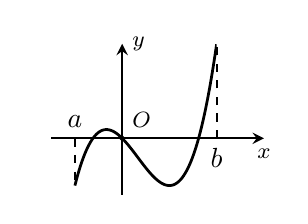
\begin{tikzpicture}[scale=0.6,thick,>=stealth, x=1.0cm,y=1.0cm]
				\draw [->] (-1.5,0)--(3,0)node[below]{\footnotesize $x$};
				\draw [->] (0,-1.2)--(0,2)node[right]{\footnotesize $y$};
				\draw [fill=white,draw=black] (0,0) circle (1pt)node[above right] {\footnotesize $O$};
				\draw [dashed](-1,0)node[above]{$a$}--(-1,-1) (2,0)node[below]{$b$}--(2,2);
				\clip(-2,-1.2) rectangle (2,2);
				\draw[line width=1.0pt,smooth,samples=100,domain=-1:2]  plot(\x,{(\x)^3-(\x)^2-(\x)});
		\end{tikzpicture}}
	\end{luuy}
\end{itemize}

\subsubsection{MỘT SỐ ĐỊNH LÝ CƠ BẢN}
\begin{itemize}
	\item [\iconMT] \indam{Định lý 1.} Giả sử $y=f(x)$ và $y=g(x)$ là hai hàm số liên tục tại điểm $x_0$. Khi đó
	\begin{gachsoc}
		\begin{itemize}
			\item Các hàm số $y=f(x)+g(x)$, $y=f(x)-g(x)$ và $y=f(x)\cdot g(x)$ liên tục tại $x_0$.
			\item Hàm số $y=\dfrac{f(x)}{g(x)}$ liên tục tại $x_0$ nếu $g(x_0)\neq 0$.
		\end{itemize}
	\end{gachsoc}
	\item [\iconMT] \indam{Định lý 2.} Sự tồn tại nghiệm của phương trình trên một khoảng
	\begin{gachsoc}
		\begin{itemize}
			\item Nếu hàm số $y=f(x)$ liên tục trên đoạn $[a;b]$ và $f(a) \cdot f(b)<0$, thì tồn tại ít nhất một điểm $c\in (a;b)$ sao cho $f(c)=0$.
			\item Nếu hàm số $y=f(x)$ liên tục trên đoạn $[a;b]$ và $f(a)\cdot f(b)<0$ thì phương trình $f(x)=0$ có ít nhất một nghiệm nằm trong khoảng $(a;b)$.
		\end{itemize}
	\end{gachsoc}
\end{itemize}

\begin{dang}{Xét tính liên tục của hàm số tại một điểm}
	Cho hàm số $y=f(x)$ xác định trên tập $D$. Để xét tính liên tục của hàm số $y=f(x)$ tại điểm $x_{0}\in D$, ta thực hiện các bước sau:
	\begin{itemize}
		\item [\iconMT] Bước 1. Tính $f(x_0)$.
		\item [\iconMT] Bước 2. Tìm $\lim\limits_{x\to x_0}f(x)$.
		\item [\iconMT] Bước 3. So sánh và rút ra kết luận.
		\begin{itemize}
			\item Nếu $\lim\limits_{x\to x_0}f(x)=f(x_0)$ thì hàm số $f(x)$ liên tục tại điểm $x_0$.
			\item Nếu $\lim\limits_{x\to x_0}f(x)\ne f(x_0)$ thì hàm số $f(x)$ không liên tục (gián đoạn) tại điểm $x_0$.
		\end{itemize}
	\end{itemize}
\end{dang}

\begin{dang}{Xét tính liên tục của hàm số trên miền xác định}
	\begin{itemize}
		\item [\iconMT] Hàm đa thức liên tục trên $\mathbb{R}$.
		\item [\iconMT] Hàm phân thức hữu tỉ, hàm lượng giác liên tục trên từng khoảng xác định của chúng.
	\end{itemize}
\end{dang}

\begin{dang}{Chứng minh phương trình có nghiệm}
	\begin{itemize}
		\item [\iconMT] Để chứng minh phương trình $f(x)=0$ có ít nhất một nghiệm trên $D$, ta chứng minh hàm số $y=f(x)$ liên tục trên $ D $ và có hai số $a,b\in D$ sao cho $f(a).f(b)<0$. 
		\item [\iconMT] Để chứng minh phương trình $f(x)=0$ có $ k $ nghiệm trên $ D $, ta chứng minh hàm số $y=f(x)$ liên tục trên $D$ và tồn tại $k$ khoảng rời nhau $(a_i;{a}_{i+1})\left(i=1,2,\ldots ,k\right)$ nằm trong $D$ sao cho $f(a_i).f({a}_{i+1})<0$.
	\end{itemize}
\end{dang}